\documentclass{beamer}
\usetheme[progressbar=frametitle]{metropolis}

\usepackage[T1]{fontenc}
\usepackage[utf8]{inputenc}
\usepackage[brazil]{babel}
\usepackage{graphicx}
\usepackage{booktabs}
\usepackage{float}

\usepackage{pifont}
\newcommand{\cmark}{\ding{51}}
\newcommand{\xmark}{\ding{55}}

\usepackage[table]{xcolor}
\usepackage{caption}

\title{Aplicação K-Means}
\subtitle{Projeto Concorrente I}
\author{Rary Emanuel Gonçalves Coringa}
\institute{
    DIM0124 - Programação Concorrente \\
    Departamento de Informática e Matemática Aplicada \\
    Universidade Federal do Rio Grande do Norte
}
\date{}

\begin{document}

\begin{frame}[plain]
    \titlepage
\end{frame}

\begin{frame}
    \frametitle{Sumário}
    \tableofcontents
\end{frame}

\section{Introdução}

\begin{frame}{Algoritmo K-Means}
    Algoritmo de agrupamento não supervisionado que particiona $N$ pontos em $k$ grupos.

    \medskip
    \textbf{Duas fases por iteração:}
    \begin{enumerate}
        \item \textbf{Atribuição} — cada ponto é atribuído ao centróide mais próximo
              (distância Euclidiana)
        \item \textbf{Atualização} — cada centróide é recomputado como a média dos seus
              pontos atribuídos
    \end{enumerate}

    \medskip
    Repete até os centróides estabilizarem (deslocamento máximo $\leq$ tolerância) ou
    \texttt{maxIter} ser atingido.

    \medskip
    \textbf{Complexidade por iteração:} $O(N \cdot k \cdot d)$
    \begin{itemize}
        \item $N$ = número de pontos \quad $k$ = clusters \quad $d$ = dimensões
    \end{itemize}
\end{frame}

\begin{frame}{Dataset e Configuração}
    \begin{columns}
        \column{0.5\textwidth}
        \textbf{Dataset}
        \begin{itemize}
            \item $\approx$5,75 milhões de linhas
            \item 38 atributos numéricos
            \item $\approx$1,75 GB em memória
            \item Pedidos de e-commerce (sintético)
        \end{itemize}

        \column{0.5\textwidth}
        \textbf{Parâmetros de agrupamento}
        \begin{itemize}
            \item $k = 10$ clusters
            \item \texttt{maxIter} = 20 (execução completa)
            \item \texttt{tolerance} = $10^{-6}$
            \item JDK 25.0.1, 16 CPUs lógicas
        \end{itemize}
    \end{columns}

    \medskip
    \begin{table}
        \centering
        \tiny
        \begin{tabular}{lrrrrrr}
            \toprule
            \textbf{order\_id} & \textbf{latitude} & \textbf{longitude} & \textbf{seller\_rating} & \textbf{shipping\_fee} & \textbf{items\_count} & \textbf{delivery\_hours} \\
            \midrule
            O-00000001 & 54.8877 & $-$1.6479 & 4.46 &  0.60 & 4 &  53 \\
            O-00000002 & 51.4400 & $-$0.0266 & 4.30 &  9.65 & 8 &  58 \\
            O-00000003 & 51.4070 & $-$2.4147 & 4.52 &  5.94 & 5 & 122 \\
            \bottomrule
        \end{tabular}
        \caption*{\scriptsize Linhas de amostra (4 colunas de ID excluídas dos atributos; 38 colunas numéricas utilizadas)}
    \end{table}
\end{frame}

\begin{frame}{Estratégia de Benchmarking}
    \begin{table}
        \centering
        \begin{tabular}{lll}
            \toprule
            \textbf{Ferramenta} & \textbf{Finalidade} & \textbf{Config} \\
            \midrule
            JCStress & Detecção de race condition & 6 forks, 5 $\times$ 1s \\
            JMH      & Microbenchmark (por operação) & 1 fork, 1wu + 3$\times$10s \\
            JMeter   & Macrobenchmark (throughput) & 120s + 30s ramp \\
            JFR      & Perfil de CPU e GC & \texttt{settings=profile} \\
            \bottomrule
        \end{tabular}
    \end{table}

    \medskip
    \begin{itemize}
        \item JMH mede custo de computação isolado (B1--B4)
        \item JMeter mede throughput do sistema sob carga concorrente
        \item JFR revela onde o tempo é efetivamente gasto
    \end{itemize}
\end{frame}

\section{Implementação Serial}

\begin{frame}{Java Serial --- Como Funciona}
    \begin{itemize}
        \item A cada iteração, o algoritmo \alert{relê o CSV do disco} inteiro
        \item Para cada linha: converte texto para números, calcula o cluster mais próximo, acumula
        \item Tudo em uma única thread --- leitura e computação misturados
    \end{itemize}

    \vspace{0.8em}
    \begin{block}{Expectativa}
        O gargalo deveria ser a aritmética do K-Means --- é ela que é executada milhões de vezes.
    \end{block}
\end{frame}

\begin{frame}{Onde o Tempo é Gasto? (JFR)}
    \begin{center}
        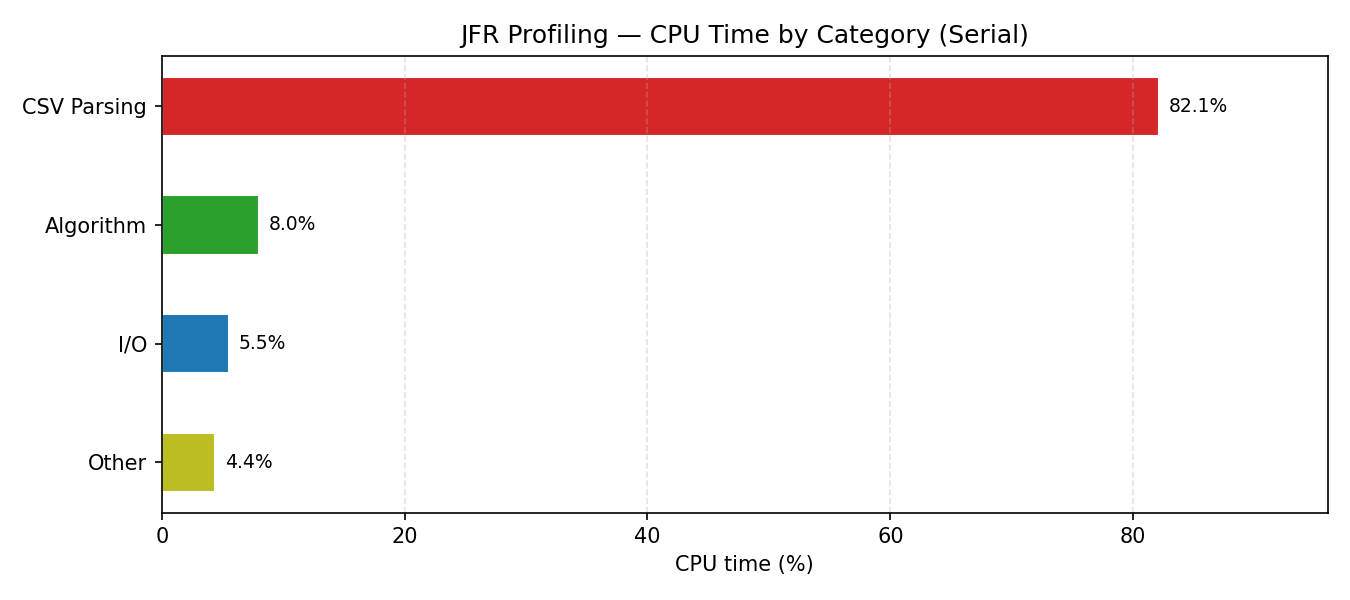
\includegraphics[width=0.82\textwidth]{img/chart4_jfr_hot_methods}
    \end{center}
    \vspace{-0.4em}
    {\small \alert{82\% do CPU} gasto convertendo texto para número --- o algoritmo em si representa apenas 8\%.}
\end{frame}

\begin{frame}{Resultados --- Serial}
    \begin{columns}
        \begin{column}{0.5\textwidth}
            \textbf{Microbenchmark (JMH)}
            \begin{itemize}
                \item Execução completa: \alert{212 s}
                \item Custo por iteração: \alert{$\approx$12 s}
                \item \texttt{closestCentroid}: 96 ns/chamada
                \item \texttt{squaredDistance}: 9 ns/chamada
            \end{itemize}
        \end{column}
        \begin{column}{0.5\textwidth}
            \textbf{Macrobenchmark (JMeter)}
            \begin{itemize}
                \item 1 thread: 1,56 exec/min
                \item 16 threads: 4,66 exec/min
                \item Ganho de $\approx$3$\times$ com 16$\times$ mais threads
                \item GC: $<$1\% do tempo total
            \end{itemize}
        \end{column}
    \end{columns}

    \vspace{0.6em}
    \begin{alertblock}{Diagnóstico}
        O gargalo não é a CPU --- é a conversão do CSV a cada iteração.
        Paralelizar a aritmética sozinha não vai ajudar.
    \end{alertblock}
\end{frame}

\begin{frame}{Comparação de Coletores de GC --- Throughput}
    Três coletores testados com 1, 2, 4, 8 e 16 threads JMeter (implementação serial):

    \vspace{0.8em}
    \begin{center}
    \begin{tabular}{lrr}
        \toprule
        \textbf{Coletor} & \textbf{1 thread} & \textbf{16 threads} \\
        \midrule
        G1GC (padrão JDK 25) & 1,56 exec/min & 4,66 exec/min \\
        ZGC                  & 1,50 exec/min & 4,40 exec/min \\
        ParallelGC           & 1,52 exec/min & \alert{4,85 exec/min} \\
        \bottomrule
    \end{tabular}
    \end{center}
\end{frame}

\begin{frame}{Comparação de Coletores de GC --- Conclusão}
    \begin{itemize}
        \item \textbf{ParallelGC} lidera levemente em alta carga --- otimizado para vazão
        \item \textbf{ZGC} fica um pouco atrás --- suas barreiras de escrita têm custo extra
        \item \textbf{G1GC} equilibrado, entre os dois
        \item Pausas de GC somam \alert{$<$1\%} do tempo em todos os casos
    \end{itemize}

    \vspace{1em}
    \begin{block}{O padrão se repete nas variantes v2}
        Coletor de GC não é o gargalo. A escolha tem impacto marginal no throughput.
    \end{block}
\end{frame}

\section{Concorrente v2 --- Lotes e Workers}

\begin{frame}{O que Mudou na v2}
    \begin{itemize}
        \item Pontos agrupados em lotes de 5.000 e distribuídos para workers em paralelo
        \item Cada worker acumula em arrays \textbf{locais} --- sem sincronização necessária
        \item Thread coordenadora reduz os resultados após todos os workers terminarem
    \end{itemize}

    \vspace{0.5em}
    Três variantes testadas:
    \begin{itemize}
        \item \textbf{v2-platform} --- workers com threads reais do sistema operacional
        \item \textbf{v2-virtual} --- workers com virtual threads (Java 21+)
        \item \textbf{v2-hybrid} --- workers reais + coordenador virtual
    \end{itemize}
\end{frame}

\begin{frame}{Resultados v2 --- Microbenchmark}
    \begin{center}
    \begin{tabular}{lrr}
        \toprule
        \textbf{Abordagem} & \textbf{B2 (s/op)} & \textbf{Erro} \\
        \midrule
        Serial       & 60,05 & $\pm$2,46 \\
        v2-platform  & 60,69 & $\pm$6,41 \\
        v2-virtual   & 71,61 & \alert{$\pm$227,05} \\
        v2-hybrid    & 60,44 & $\pm$5,33 \\
        \bottomrule
    \end{tabular}
    \end{center}

    \vspace{0.5em}
    \begin{alertblock}{Nenhuma melhoria no tempo por iteração}
        A leitura sequencial do CSV continua dominando. Paralelizar apenas a aritmética
        (8\% do tempo) não move o resultado.
    \end{alertblock}
\end{frame}

\begin{frame}{Resultados v2 --- Macrobenchmark por Coletor}
    Throughput por coletor de GC (v2-platform, mesma tendência nas outras variantes):

    \vspace{0.6em}
    \begin{center}
    \begin{tabular}{lrr}
        \toprule
        \textbf{Coletor} & \textbf{1 thread} & \textbf{16 threads} \\
        \midrule
        G1GC       & 1,65 exec/min & 4,49 exec/min \\
        ZGC        & 1,41 exec/min & 4,13 exec/min \\
        ParallelGC & 1,60 exec/min & 4,39 exec/min \\
        \bottomrule
    \end{tabular}
    \end{center}

    \vspace{0.6em}
    ZGC levemente atrás, ParallelGC e G1GC equivalentes --- \alert{mesmo padrão da versão serial}.
    Nenhum coletor resolve o gargalo real: a leitura do CSV.
\end{frame}

\begin{frame}{Resultados v2 --- Condições de Corrida (JCStress)}
    \begin{itemize}
        \item Leituras concorrentes dos centróides: \textcolor{green!60!black}{\cmark\ seguras}
        \item Escrita em array compartilhado sem proteção: \textcolor{red}{\xmark\ até 28\% de atualizações perdidas}
        \item Solução adotada: cada worker acumula em arrays próprios
    \end{itemize}

    \vspace{1em}
    \begin{block}{Insight da v2-hybrid}
        O coordenador virtual suspende durante leitura de arquivo, tornando o CSV
        invisível ao profiler --- revelando que o problema era a leitura, não a coordenação.
    \end{block}
\end{frame}

\section{Concorrente v3 --- Dados em Memória}

\begin{frame}{A Mudança Decisiva}
    \begin{alertblock}{Problema identificado}
        A cada iteração, o algoritmo relê e converte $\approx$1 GB de CSV.
        Isso acontece 3 a 20 vezes por execução.
    \end{alertblock}

    \vspace{0.5em}
    \textbf{Solução:} carregar todo o dataset em memória \alert{uma única vez} antes das iterações.

    \vspace{0.5em}
    \begin{itemize}
        \item Dataset lido na inicialização e mantido como array de doubles
        \item Iterações operam diretamente sobre o array --- sem disco
        \item Array dividido em $N$ partes (uma por processador lógico)
        \item Workers processam em paralelo, coordenador aguarda todos com \texttt{CountDownLatch}
    \end{itemize}
\end{frame}

\begin{frame}{Resultados v3 --- Microbenchmark}
    \begin{itemize}
        \item Custo por iteração: 60 s $\to$ \alert{1,6 s} (\alert{37$\times$} mais rápido)
        \item Variância colapsa: $\pm$227 s $\to$ $\pm$0,17 s --- iterações previsíveis
        \item Perfil JFR: nenhum evento de leitura de arquivo durante o clustering
    \end{itemize}

    \vspace{0.8em}
    \textbf{Trade-off de memória}
    \begin{itemize}
        \item Heap: 250 MB $\to$ \alert{2,7 GB}
        \item GC: 1.000 coletas $\to$ apenas 60 coletas
        \item Dataset precisa caber inteiro na RAM
    \end{itemize}
\end{frame}

\begin{frame}{Resultados v3 --- Macrobenchmark}
    \begin{itemize}
        \item 1 thread JMeter: 1,6 $\to$ \alert{52,5 exec/min} (\alert{32$\times$})
        \item 16 threads JMeter: 4,5 $\to$ \alert{62,3 exec/min} (\alert{14$\times$})
    \end{itemize}

    \vspace{0.8em}
    \begin{block}{Por que o ganho diminui com mais threads?}
        Com tudo em memória, cada execução já ocupa todos os núcleos internamente.
        Threads JMeter adicionais competem pelos mesmos recursos.
    \end{block}

    \vspace{0.5em}
    \begin{alertblock}{Comparação direta com a versão serial}
        Serial: 1,56 exec/min com 1 thread \quad$\to$\quad v3: 52,5 exec/min com 1 thread
    \end{alertblock}
\end{frame}

\section{Implementação Erlang}

\begin{frame}{Por que Não há Versão Serial}
    \begin{itemize}
        \item Erlang é construída em torno do modelo de atores: processos são a
              unidade fundamental de execução
        \item Toda computação significativa acontece por troca de mensagens
        \item Escrever um K-Means verdadeiramente serial forçaria a ignorar os
              mecanismos centrais da linguagem
    \end{itemize}

    \vspace{0.5em}
    \begin{block}{Decisão}
        A implementação Erlang parte diretamente da versão concorrente com dados em memória,
        o equivalente à v3 em Java.
    \end{block}
\end{frame}

\begin{frame}{Como Funciona --- Modelo de Atores}
    \begin{itemize}
        \item Dataset em memória, \alert{16 workers} BEAM --- um por scheduler disponível
        \item Cada worker mantém seu pedaço dos dados localmente desde a inicialização
    \end{itemize}

    \vspace{0.5em}
    \textbf{A cada iteração:}
    \begin{enumerate}
        \item Processo principal envia os centróides para cada worker
        \item Workers calculam o cluster mais próximo e acumulam resultados parciais
        \item Workers enviam os parciais de volta ao processo principal
        \item Processo principal agrega e recalcula os centróides
    \end{enumerate}
\end{frame}

\begin{frame}{Resultados Erlang vs Java v3}
    \begin{center}
    \begin{tabular}{lrrr}
        \toprule
        \textbf{Benchmark} & \textbf{Java v3} & \textbf{Erlang} & \textbf{Fator} \\
        \midrule
        \texttt{closestCentroid} & 96 ns & 15.976 ns & \alert{165$\times$} \\
        \texttt{squaredDistance} & 9 ns  &  1.053 ns & \alert{113$\times$} \\
        5 iterações completas    & 1,6 s & 106,3 s   & \alert{66$\times$} \\
        \bottomrule
    \end{tabular}
    \end{center}

    \vspace{0.8em}
    Ambas as implementações usam dados em memória e 16 workers. \\
    A diferença é inteiramente na \alert{velocidade da aritmética por ponto}.
\end{frame}

\begin{frame}{Por que Erlang é Mais Lento?}
    \begin{itemize}
        \item \textbf{Aritmética:} JVM otimiza loops com vetorização SIMD; BEAM processa cada valor individualmente
        \item \textbf{Ociosidade:} schedulers com \alert{45,7\%} de utilização --- workers ficam parados enquanto o processo principal agrega os resultados
        \item \textbf{GC:} \alert{2,13 milhões} de coletas (Erlang) vs \alert{60} (Java) --- cada ponto processado gera objetos temporários na BEAM
    \end{itemize}

    \vspace{0.8em}
    \begin{block}{Estrutural, não acidental}
        Esses custos são inerentes ao modelo de atores para cargas CPU-bound.
        Erlang não foi projetada para este tipo de workload.
    \end{block}
\end{frame}

\section{Comparativo Final}

\begin{frame}{Custo por Iteração --- Todas as Abordagens}
    \begin{center}
        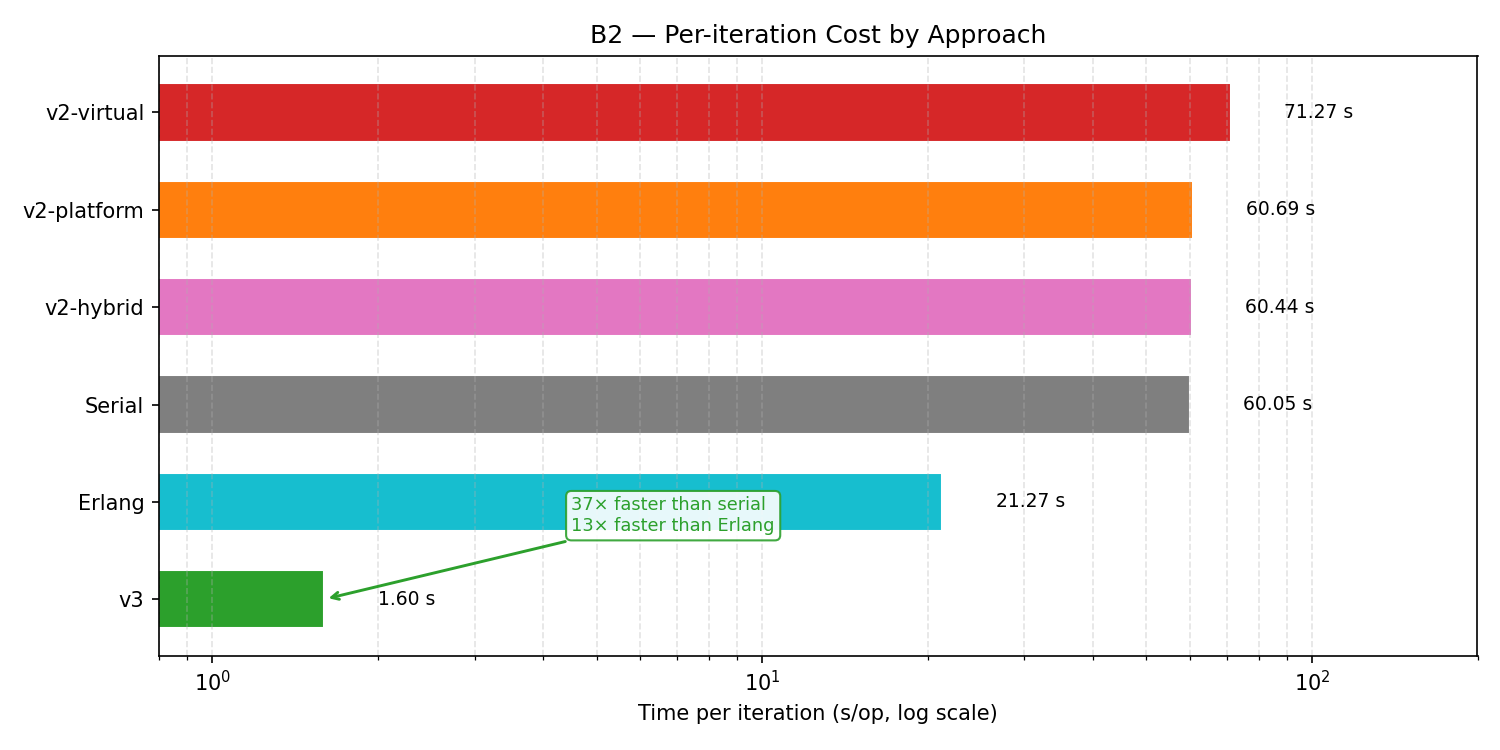
\includegraphics[width=0.90\textwidth]{img/chart1_b2_cost}
    \end{center}
\end{frame}

\begin{frame}{Evolução do Throughput}
    \begin{center}
        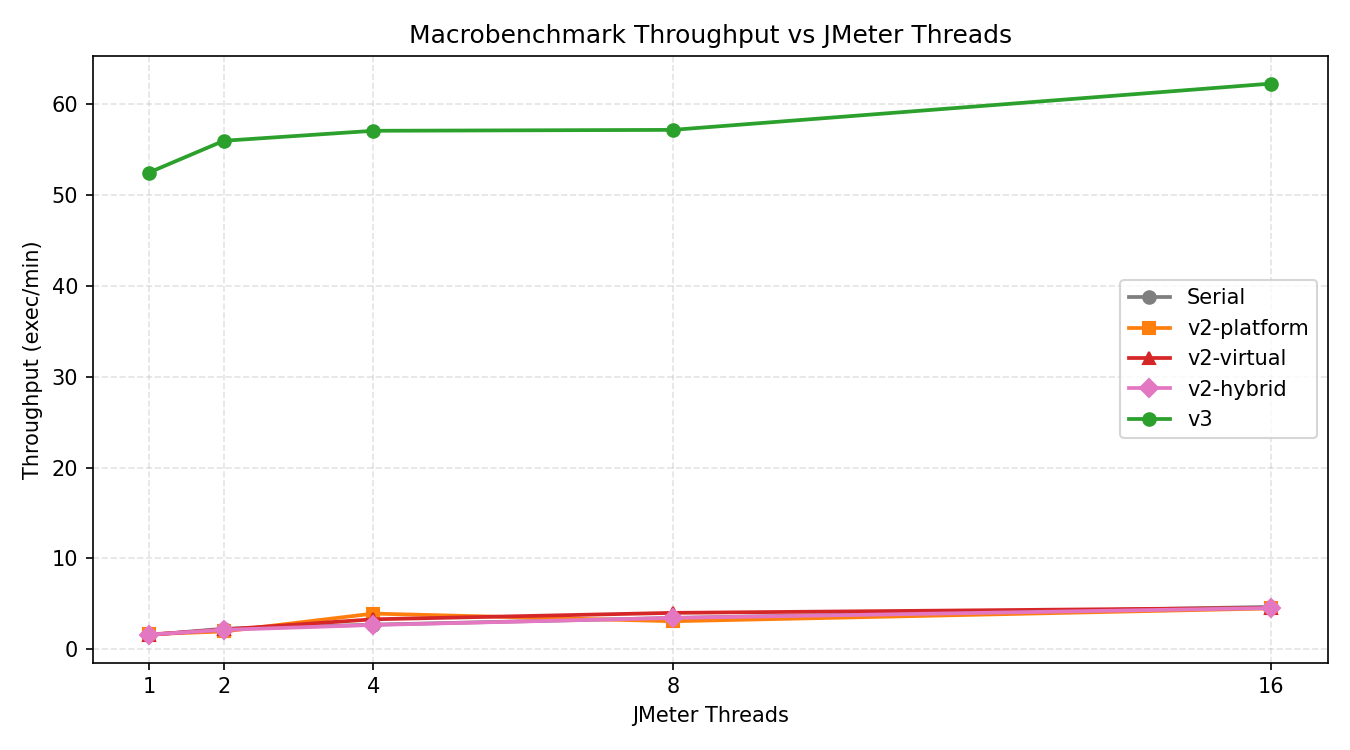
\includegraphics[width=0.90\textwidth]{img/chart2_macro_throughput}
    \end{center}
    {\small Painel superior: Serial e v2 (escala 0--7). Painel inferior: v3 (escala 0--70).}
\end{frame}

\begin{frame}{Trade-off: Releitura do CSV vs Dados em Memória}
    \begin{columns}
        \begin{column}{0.48\textwidth}
            \textbf{Releitura a cada iteração (v1/v2)}
            \begin{itemize}
                \item[\cmark] Baixo consumo de memória ($\approx$250 MB)
                \item[\cmark] Dataset pode ser maior que a RAM
                \item[\xmark] 82\% do CPU gasto em conversão de texto
                \item[\xmark] $\approx$12 s por iteração
            \end{itemize}
        \end{column}
        \begin{column}{0.48\textwidth}
            \textbf{Dataset em memória (v3)}
            \begin{itemize}
                \item[\cmark] Iterações 37$\times$ mais rápidas
                \item[\cmark] CPU dedicado 100\% ao algoritmo
                \item[\xmark] Heap de $\approx$2,7 GB necessário
                \item[\xmark] Dataset deve caber na RAM
            \end{itemize}
        \end{column}
    \end{columns}

    \vspace{0.5em}
    \begin{alertblock}{Lição}
        O JFR revelou onde o tempo realmente ia. Sem medir, paralelizaríamos
        os 8\% do algoritmo e ignoraríamos os 82\% do CSV.
    \end{alertblock}
\end{frame}

\begin{frame}{Quando Cada Modelo Vence}
    \begin{columns}
        \begin{column}{0.48\textwidth}
            \textbf{Java (memória compartilhada)}
            \begin{itemize}
                \item[\cmark] Aritmética 113--165$\times$ mais rápida
                \item[\cmark] Todos os núcleos ativos durante iteração
                \item[\cmark] Muito menos pressão de GC
                \item[$\cdot$] Ideal para cargas CPU-bound
            \end{itemize}
        \end{column}
        \begin{column}{0.48\textwidth}
            \textbf{Erlang (modelo de atores)}
            \begin{itemize}
                \item[\cmark] Race conditions impossíveis por construção
                \item[\cmark] GC sem pausas globais
                \item[\cmark] Escala para sistemas distribuídos
                \item[$\cdot$] Ideal para I/O intensivo e alta disponibilidade
            \end{itemize}
        \end{column}
    \end{columns}

    \vspace{0.5em}
    K-Means é CPU-bound com pouca comunicação entre iterações ---
    \alert{o caso em que memória compartilhada tem vantagem estrutural}.
\end{frame}


\begin{frame}[standout]
    \centering \huge{Obrigado!}
\end{frame}

\end{document}
